\documentclass[a4paper, 11pt]{article}

%Comandos para configurar el idioma
\usepackage[spanish,activeacute]{babel}
\usepackage[utf8]{inputenc}
\usepackage[T1]{fontenc} %Necesario para el uso de las comillas latinas.
\usepackage{geometry}
\usepackage{graphicx}

%Importante que esta sea la última órden del preámbulo
\usepackage{hyperref}

\newcommand\fnurl[2]{%
  \href{#2}{#1}\footnote{\url{#2}}%
}

\newcommand{\includecode}[2][c]{\lstinputlisting[caption=#2, escapechar=, style=custom#1]{#2}<!---->}

%Paquetes matemáticos
\usepackage{amsmath,amsfonts,amsthm}
\usepackage[all]{xy} %Para diagramas
\usepackage{enumerate} %Personalización de enumeraciones
\usepackage{tikz} %Dibujos

%Tipografía escalable
\usepackage{lmodern}
%Legibilidad
\usepackage{microtype}

%Código
\usepackage{listings}
\usepackage{color}

\definecolor{dkgreen}{rgb}{0,0.6,0}
\definecolor{gray}{rgb}{0.5,0.5,0.5}
\definecolor{mauve}{rgb}{0.58,0,0.82}

\definecolor{listinggray}{gray}{0.9}
\definecolor{lbcolor}{rgb}{0.9,0.9,0.9}
\lstset{
backgroundcolor=\color{lbcolor},
    tabsize=4,
rulecolor=,
    language=[GNU]C++,
        basicstyle=\scriptsize,
        upquote=true,
        aboveskip={1.5\baselineskip},
        columns=fixed,
        showstringspaces=false,
        extendedchars=false,
        breaklines=true,
        prebreak = \raisebox{0ex}[0ex][0ex]{\ensuremath{\hookleftarrow}},
        frame=single,
        numbers=left,
        showtabs=false,
        showspaces=false,
        showstringspaces=false,
        identifierstyle=\ttfamily,
        keywordstyle=\color[rgb]{0,0,1},
        commentstyle=\color[rgb]{0.026,0.112,0.095},
        stringstyle=\color[rgb]{0.627,0.126,0.941},
        numberstyle=\color[rgb]{0.205, 0.142, 0.73},
%        \lstdefinestyle{C++}{language=C++,style=numbers}’.
}
\lstset{
    backgroundcolor=\color{lbcolor},
    tabsize=4,
  language=C++,
  captionpos=b,
  tabsize=3,
  frame=lines,
  numbers=left,
  numberstyle=\tiny,
  numbersep=5pt,
  breaklines=true,
  showstringspaces=false,
  basicstyle=\footnotesize,
%  identifierstyle=\color{magenta},
  keywordstyle=\color[rgb]{0,0,1},
  commentstyle=\color[rgb]{0.026,0.112,0.095}, % Darkgreen
  stringstyle=\color{red}
  }
% Slightly bigger margins than the latex defaults

\geometry{verbose,tmargin=1in,bmargin=1in,lmargin=1in,rmargin=1in}
\setlength{\parskip}{.5em} % por defecto el espacio entre párrafos es 0pt

\theoremstyle{definition}
\newtheorem{ejercicio}{Ejercicio}
\newtheorem{cuestion}{Cuestión}
\newtheorem*{solucion}{Solución}
\newtheorem*{bonus}{BONUS}

%%%%%%%% New sqrt
\usepackage{letltxmacro}
\makeatletter
\let\oldr@@t\r@@t
\def\r@@t#1#2{%
\setbox0=\hbox{$\oldr@@t#1{#2\,}$}\dimen0=\ht0
\advance\dimen0-0.2\ht0
\setbox2=\hbox{\vrule height\ht0 depth -\dimen0}%
{\box0\lower0.4pt\box2}}
\LetLtxMacro{\oldsqrt}{\sqrt}
\renewcommand*{\sqrt}[2][\ ]{\oldsqrt[#1]{#2} }
\makeatother

%%%%%%%%%%%%%%%%%%%%%%%%%%%%%%%%%%%%%%%%%%%

\hypersetup{
  pdftitle={Informe de trabajo 2},
  pdfauthor={Antonio Álvarez Caballero},
  unicode,
  breaklinks=true,  % so long urls are correctly broken across lines
  colorlinks=true,
  urlcolor=blue,
  linkcolor=blue,
  citecolor=darkgreen,
  }

\title{Informe de trabajo 2}
\author{Antonio Álvarez Caballero\\
    \href{mailto:analca3@correo.ugr.es}{analca3@correo.ugr.es}}
\date{}
%%%%%%%%%%%%%%%%% FIN PREAMBULO %%%%%%%%%%%%%%%%%%%%%%%%%%%

\begin{document}

  \maketitle

  \section{Estimación de una homografía}

    La primera parte de la práctica consiste en estimar una homografía según dos
    conjuntos de puntos y aplicársela a una imagen para llevárnosla al mismo plano que la segunda.
    Usaremos las imágenes del tablero para realizar este ejercicio.

    \subsection{Selección de puntos}

      Primero debemos seleccionar $10$ puntos a mano en correspondencia en cada uno de los tableros.
      Después de varias pruebas de ensayo y error (poner los puntos medianamente simétricos no es una opción muy buena),
      se escogen los puntos marcados en azul en la figura resultado.
      Con esos puntos se consigue una buena homografía, las pruebas las he hecho poniendo una
      imagen sobre otra, coincidiendo los cuadrados negros del tablero.

      \begin{lstlisting}
        // Taking points by hand
        vector<Point> origin, destination;

        origin.push_back(Point(156,  49));
        origin.push_back(Point(530,  13));
        origin.push_back(Point(215,  90));
        origin.push_back(Point(474, 103));
        origin.push_back(Point(362, 134));
        origin.push_back(Point(305, 330));
        origin.push_back(Point(184, 348));
        origin.push_back(Point(438, 397));
        origin.push_back(Point(137, 422));
        origin.push_back(Point(527, 464));

        destination.push_back(Point(148,  14));
        destination.push_back(Point(502,  96));
        destination.push_back(Point(212,  80));
        destination.push_back(Point(446, 157));
        destination.push_back(Point(347, 160));
        destination.push_back(Point(264, 322));
        destination.push_back(Point(138, 323));
        destination.push_back(Point(374, 386));
        destination.push_back(Point(76 , 387));
        destination.push_back(Point(431, 443));
      \end{lstlisting}

    \subsection{Estimación de la homografía y transformación}

      Para estimar la homografía se usa lo visto en clase. Formamos una matriz con los
      coeficientes de las ecuaciones que debemos resolver para conseguir la homografía
      (salen $2n \times 9$ ecuaciones, siendo $n$ el número de puntos), y posteriormente
      para resolver dicho sistema utilizamos la $SVD$. El vector singular asociado al valor
      singular más pequeño será la solución buscada. Sólo tendremos que organizarlo como una matriz $3 \times 3$.

      Dejo el código usado para tal fin. Se ha creado una clase homografía con el único
      propósito de restringir el tipo de dato que le entra a la función \textit{warpPerspective}
      que he creado en la clase \textit{Image} para aplicar la homografía a la imagen.

      \begin{lstlisting}
        Mat Homography::homographyEquationMatrix(vector<Point> origin, vector<Point> destination)
        {
          // Check input size
          if (origin.size() != destination.size())
          {
            return Mat::zeros(3,3,CV_32FC1);
          }

          int num_points = origin.size();
          int num_equations = 2 * num_points;

          // Fill new matrix with zeros
          Mat coeffs = Mat::zeros(num_equations, 9, CV_32FC1);

          Point ori, dest;

          // Set coeffs of the equation matrix as slides
          for (int i = 0; i < num_points; i++)
          {
            ori = origin[i];
            dest = destination[i];

            int actual_row = 2 * i;
            int next_row = actual_row + 1;

            coeffs.at<float>(Point(0,actual_row)) = ori.x;
            coeffs.at<float>(Point(1,actual_row)) = ori.y;
            coeffs.at<float>(Point(2,actual_row)) = 1;
            coeffs.at<float>(Point(6,actual_row)) = -dest.x * ori.x;
            coeffs.at<float>(Point(7,actual_row)) = -dest.x * ori.y;
            coeffs.at<float>(Point(8,actual_row)) = -dest.x;

            coeffs.at<float>(Point(3,next_row)) = ori.x;
            coeffs.at<float>(Point(4,next_row)) = ori.y;
            coeffs.at<float>(Point(5,next_row)) = 1;
            coeffs.at<float>(Point(6,next_row)) = -dest.y * ori.x;
            coeffs.at<float>(Point(7,next_row)) = -dest.y * ori.y;
            coeffs.at<float>(Point(8,next_row)) = -dest.y;
          }

          return coeffs;
        }

        Mat Homography::calcHomography(vector<Point> origin, vector<Point> destination)
        {
          // Compute matrix with equation coefficients
          Mat A = homographyEquationMatrix(origin,destination);

          // Compute SVD of A (http://docs.opencv.org/master/df/df7/classcv_1_1SVD.html#a76f0b2044df458160292045a3d3714c6)
          Mat w, u, vt;
        	SVD::compute(A, w, u, vt);

          // Take last col of vt matrix and reorder as 3x3 matrix
          Mat homography_matrix = Mat(3, 3, CV_32FC1);
        	for (int i = 0; i < 3; i++)
          {
            for (int j = 0; j < 3; j++)
            {
        		  homography_matrix.at<float>(Point(j, i)) = vt.at<float>(Point(3*i + j, vt.cols -1 ));
            }
        	}

          return homography_matrix;
        }

        Homography::Homography(vector<Point> origin, vector<Point> destination)
        {
          this->homography = this->calcHomography(origin,destination);
        }

        Mat Homography::getHomography()
        {
          return homography;
        }
      \end{lstlisting}


      El siguiente paso es aplicar dicha homografía a la primera imagen para obtenerla
      con la misma proyección que la segunda. Para ello sólo debemos llamar a \textit{warpPerspective}
      con la homografía calculada anteriormente sobre la imagen base. Así conseguiremos la imagen deseada.

      \begin{lstlisting}
        Image Image::warpPerspective(Homography hom)
        {
          Mat output;

          // Using OpenCV warpPerspective with the image
          cv::warpPerspective(this->image, output, hom.getHomography(), Size(output.cols, output.rows));

          return Image(output, this->name + " warped");
        }
      \end{lstlisting}

      \begin{lstlisting}
        // Making homography using SVD
        Homography hom(origin, destination);
      	Image output_good = input.warpPerspective(hom);
      \end{lstlisting}

    \subsection{Escoger puntos malos y conclusiones}

      Ahora escogemos $10$ puntos en correspondencia agrupados en una esquina, y aplicamos lo mismo.
      Estos puntos los he coloreado de color rojo.

      \begin{lstlisting}
        // Another homography using bad points
        vector<Point> another_origin, another_destination;

      	another_origin.push_back(Point(156,  47));
      	another_origin.push_back(Point(177,  46));
      	another_origin.push_back(Point(155,  72));
      	another_origin.push_back(Point(175,  70));
      	another_origin.push_back(Point(198,  43));
      	another_origin.push_back(Point(197,  67));
      	another_origin.push_back(Point(219,  66));
      	another_origin.push_back(Point(153,  95));
      	another_origin.push_back(Point(152, 120));
      	another_origin.push_back(Point(173, 119));

      	another_destination.push_back(Point(150, 14));
      	another_destination.push_back(Point(174, 19));
      	another_destination.push_back(Point(142, 40));
      	another_destination.push_back(Point(167, 46));
      	another_destination.push_back(Point(198, 24));
      	another_destination.push_back(Point(191, 51));
      	another_destination.push_back(Point(217, 56));
      	another_destination.push_back(Point(137, 63));
      	another_destination.push_back(Point(131, 90));
      	another_destination.push_back(Point(157, 95));

        Homography hom2(another_origin, another_destination);
      	Image output_bad = input.warpPerspective(hom2);
      \end{lstlisting}

      Ahora coloreamos los puntos como hemos indicado, dibujamos todas las imágenes en un canvas y vemos los resultados.

      \begin{lstlisting}
        // Drawing circles on the selected points.
        // Blue points are good ones, red are bad ones
        int circle_radius = 10;
        int circle_thickness = 3;

        for (int i = 0; i < origin.size(); i++)
        {
          input.drawCircle(origin[i], circle_radius, Scalar(255,0,0), circle_thickness);
          dest.drawCircle(destination[i], circle_radius, Scalar(255,0,0), circle_thickness);
        }

        for (int i = 0; i < another_origin.size(); i++)
        {
          input.drawCircle(another_origin[i], circle_radius, Scalar(0,0,255), circle_thickness);
          dest.drawCircle(another_destination[i], circle_radius, Scalar(0,0,255), circle_thickness);
        }

        // Drawing canvas with all images

        vector<Image*> sequence;
        sequence.push_back(&input);
        sequence.push_back(&dest);
        sequence.push_back(&output_good);
        sequence.push_back(&output_bad);

        Image canvas(sequence, 2, 2);
        canvas.paint();

        waitKey(0);
        destroyAllWindows();
      \end{lstlisting}

      Los resultados son estos.

      \centerline{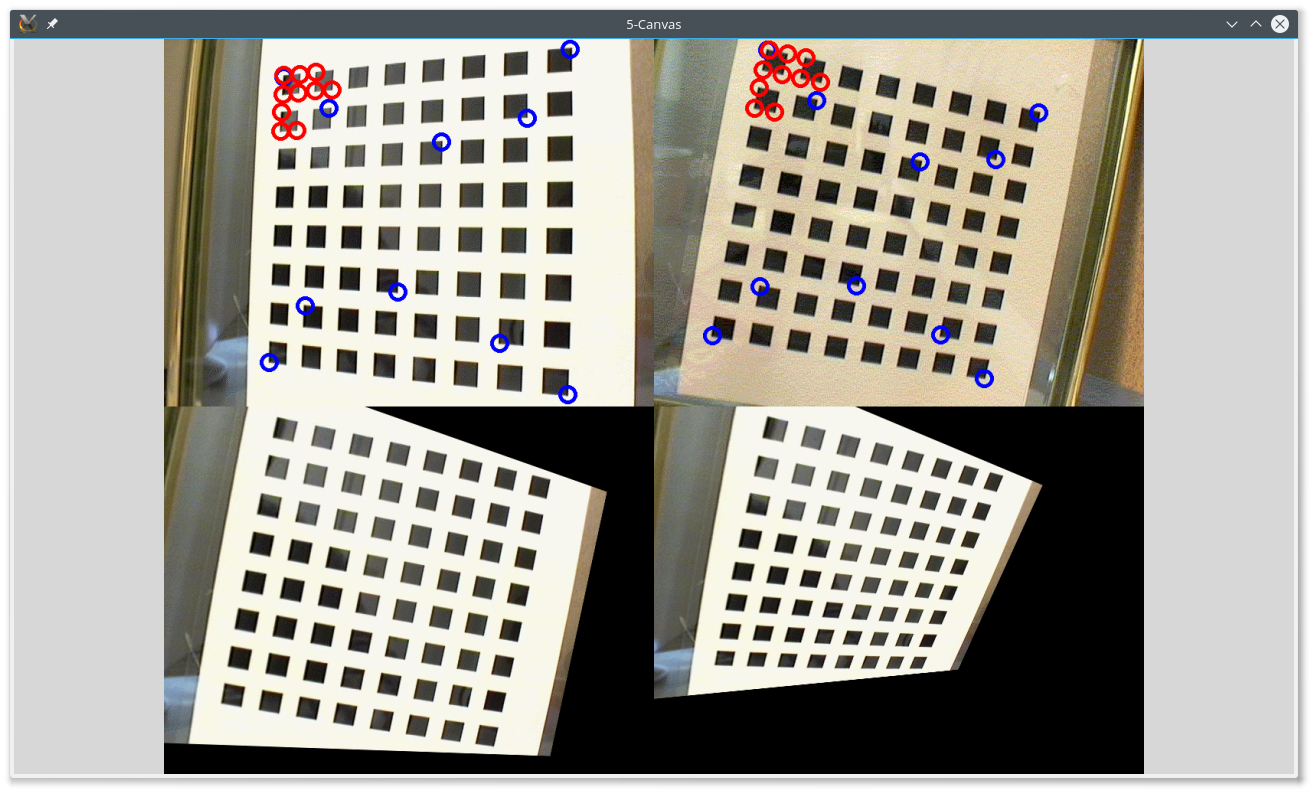
\includegraphics[width=0.7\textwidth]{Homography.png}}

      La primera fila corresponde a las imágenes origen y destino. La segunda fila consta
      de la imagen creada a partir de los puntos azules (buenos) y por puntos malos, en ese orden.

      Como se ve, la imagen formada a partir de los puntos buenos es mucho más parecida a la imagen
      destino que la que tiene todos los puntos agrupados en una esquina. Si dibujamos la imagen transformada buena
      y la destino en ventanas separadas y ponemos una encima de la otra, vemos que los cuadrados
      del tablero coinciden perfectamente, por lo que podemos deducir que la homografía estimada es buena.


  \section{Detección de regiones relevantes y cálculo de descriptores}

    En esta parte de la práctica tenemos que, usando los detectores \textit{BRISK}
    y \textit{ORB}, detectar las regiones relevantes de las imágenes de \textit{Yosemite} $1$ y $2$.
    Además tenemos que calcular sus descriptores en cada \textit{KeyPoint}.

    En esta parte de la práctica he escrito código sin usar mi diseño orientado a objetos.
    Esto es debido a que primero he probado todas las posibilidades descritas en el guión y
    cuando saque conclusiones, añadiré a mi clase imagen lo que mejor resultados me haya dado.

    Es probable que para distintas imágenes, distintos métodos funciones mejor que otros,
    pero no es objeto de estas prácticas tener algo tan general y que oscurezca el código y complique
    demasiado el desarrollo.

    Sólo tenemos que revisar la documentación de OpenCV para hacer el ejercicio, ya que nos lo da todo
    hecho. Declarar detectores, variables de salida y llamar a las funciones clave. Después, se pintan las regiones relevantes.
    Las de \textit{BRISK} se pintan en azul y las de \textit{ORB} en rojo.

    Los parámetros usados en \textit{BRISK} están basados en los que vienen por defecto,
    pero tocados un poco para que tome algunos puntos relevantes más.

    \begin{lstlisting}
      /* Excersice 2 */
      Mat im = imread("imagenes/yosemite1.jpg");
      Mat im_2 = imread("imagenes/yosemite2.jpg");

      Mat im_copy = im.clone();
      Mat im_2_copy = im_2.clone();

      vector<KeyPoint> keypointsA[2], keypointsB[2];
      Mat descriptorsA[2], descriptorsB[2];

      int Threshl=65;
      int Octaves=3;
      float PatternScales=1.0f;

      circle_radius = 5;
      circle_thickness = 1;

      /* BRISK */
      Ptr<BRISK> ptrBrisk = BRISK::create(Threshl,Octaves,PatternScales);

      ptrBrisk->detect(im, keypointsA[0]);
      ptrBrisk->compute(im, keypointsA[0],descriptorsA[0]);

      ptrBrisk->detect(im_2, keypointsA[1]);
      ptrBrisk->compute(im_2, keypointsA[1],descriptorsA[1]);

      for (int i = 0; i < keypointsA[0].size(); i++)
      {
        circle(im,keypointsA[0][i].pt, circle_radius, Scalar(255,0,0), circle_thickness);
      }

      for (int i = 0; i < keypointsA[1].size(); i++)
      {
        circle(im_2,keypointsA[1][i].pt, circle_radius, Scalar(255,0,0), circle_thickness);
      }

      /* ORB */
      Ptr<ORB> ptrORB = ORB::create();

      ptrORB->detect(im_copy, keypointsB[0]);
      ptrORB->compute(im_copy, keypointsB[0],descriptorsB[0]);

      ptrORB->detect(im_2_copy, keypointsB[1]);
      ptrORB->compute(im_2_copy, keypointsB[1],descriptorsB[1]);

      for (int i = 0; i < keypointsB[0].size(); i++)
      {
        circle(im_copy,keypointsB[0][i].pt, circle_radius, Scalar(0,0,255), circle_thickness);
      }

      for (int i = 0; i < keypointsB[1].size(); i++)
      {
        circle(im_2_copy,keypointsB[1][i].pt, circle_radius, Scalar(0,0,255), circle_thickness);
      }

      namedWindow("Brisk1", WINDOW_NORMAL);
      namedWindow("Brisk2", WINDOW_NORMAL);

      imshow("Brisk1", im);
      imshow("Brisk2", im_2);

      waitKey(0);
      destroyAllWindows();

      namedWindow("ORB1", WINDOW_NORMAL);
      namedWindow("ORB2", WINDOW_NORMAL);

      imshow("ORB1",im_copy);
      imshow("ORB2",im_2_copy);
      waitKey(0);
      destroyAllWindows();
    \end{lstlisting}

    Ahora ponemos el resultado

    \centerline{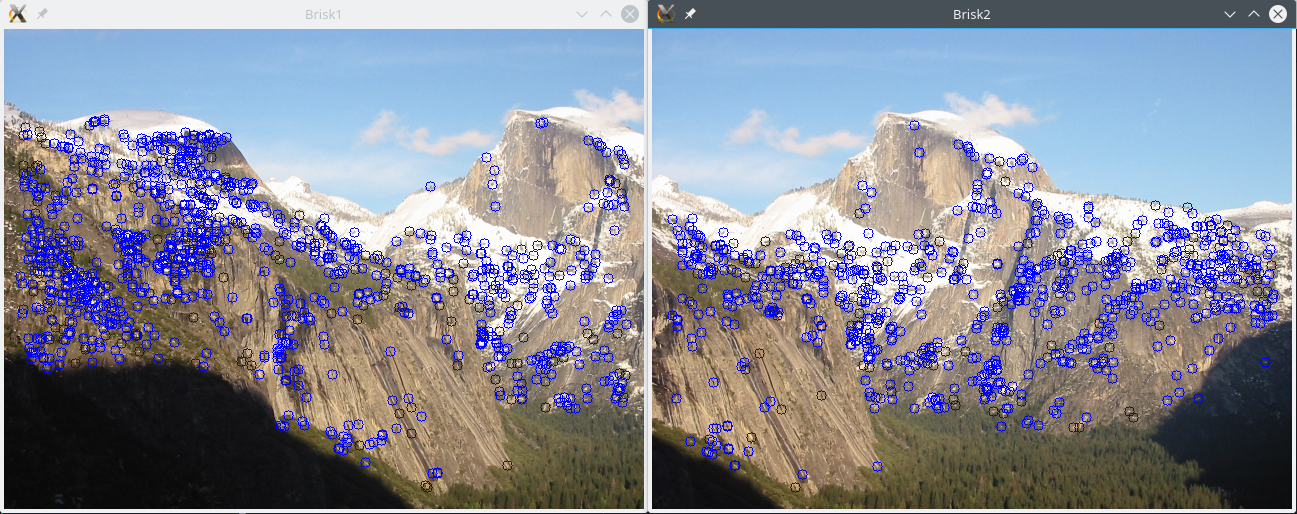
\includegraphics[width=0.7\textwidth]{BRISK.png}}
    \centerline{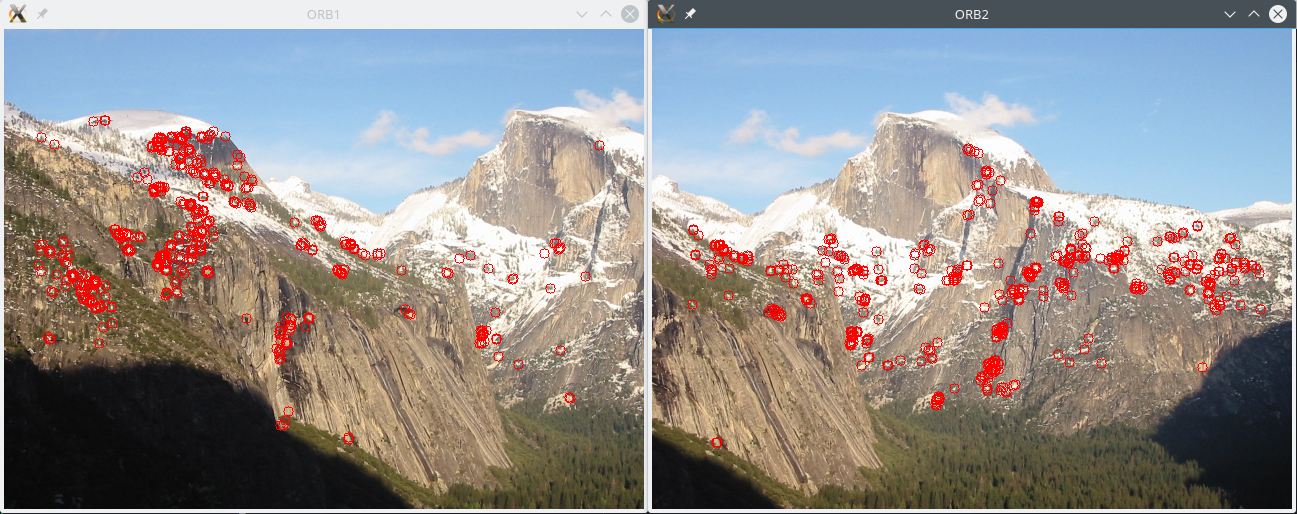
\includegraphics[width=0.7\textwidth]{ORB.png}}

    En nuestro caso nos decidimos por $BRISK$, ya que ofrece más puntos de referencia
    además de, en mi opinión, más importantes, como el pico de la montaña o la ladera junto a los árboles.

    \subsection{Cálculo de correspondencias}

      Ahora debemos calcular las correspondencias entre ambas imágenes. Aún seguimos trabajando con ambos detectores.

      Al igual que antes, sólo tenemos que usar la potencia de OpenCV. Algunas cosas a comentar:

      \begin{itemize}
        \item Los descriptores se transforman a \textit{CV\_32F} para tener compatibilidad con \textit{FlannBasedMatcher}.
        \item Para \textit{BFMatcher} se utiliza \textit{NORM\_HAMMING} según recomendación de la \fnurl{documentación}{http://docs.opencv.org/master/d3/da1/classcv_1_1BFMatcher.html\#abe0bb11749b30d97f60d6ade665617bd}
        \item Los argumentos opcionales pasados a \textit{drawMatches} son todos por defecto excepto el último \textit{DrawMatchesFlags::NOT\_DRAW\_SINGLE\_POINTS}, que sirve para no dibujar los KeyPoints sin correspondencias.
      \end{itemize}

      \begin{lstlisting}
        /* Excersice 3 */

        /* BFMatcher */
        BFMatcher BFmatcherBRISK(NORM_HAMMING, true);
        BFMatcher BFmatcherORB(NORM_HAMMING, true);

        vector<DMatch> BFmatchesBRISK, BFmatchesORB;

        // Match!
        BFmatcherBRISK.match(descriptorsA[0], descriptorsA[1], BFmatchesBRISK);
        BFmatcherORB.match(descriptorsB[0], descriptorsB[1], BFmatchesORB);


        // Draw matches
        // All parameters are the default ones but no DrawMatchesFlags::NOT_DRAW_SINGLE_POINTS
        // It prevents drawing keypoints without matches.
        Mat BFall_matchesBRISK, BFall_matchesORB;
        drawMatches( im, keypointsA[0], im_2, keypointsA[1],
                             BFmatchesBRISK, BFall_matchesBRISK, Scalar::all(-1), Scalar::all(-1),
                             vector<char>(),DrawMatchesFlags::NOT_DRAW_SINGLE_POINTS );

        drawMatches( im_copy, keypointsB[0], im_2_copy, keypointsB[1],
                            BFmatchesORB, BFall_matchesORB, Scalar::all(-1), Scalar::all(-1),
                            vector<char>(),DrawMatchesFlags::NOT_DRAW_SINGLE_POINTS );


        imshow( "BRISK All Matches BFMatcher", BFall_matchesBRISK );
        imshow( "ORB All Matches BFMatcher", BFall_matchesORB );
        waitKey(0);
        destroyAllWindows();

        /* FlannBasedMatcher */

        FlannBasedMatcher FlmatcherBRISK;
        FlannBasedMatcher FlmatcherORB;

        vector<DMatch> FlmatchesBRISK, FlmatchesORB;

        // Neccesary for FlannBasedMatcher!
        for (int i = 0; i < 2; i++)
        {
          descriptorsA[i].convertTo(descriptorsA[i], CV_32F);
        }

        for (int i = 0; i < 2; i++)
        {
          descriptorsB[i].convertTo(descriptorsB[i], CV_32F);
        }

        FlmatcherBRISK.match(descriptorsA[0], descriptorsA[1], FlmatchesBRISK);

        FlmatcherORB.match(descriptorsB[0], descriptorsB[1], FlmatchesORB);

        Mat Flall_matchesBRISK, Flall_matchesORB;
        drawMatches( im, keypointsA[0], im_2, keypointsA[1],
                             FlmatchesBRISK, Flall_matchesBRISK, Scalar::all(-1), Scalar::all(-1),
                             vector<char>(),cv::DrawMatchesFlags::NOT_DRAW_SINGLE_POINTS );

        drawMatches( im_copy, keypointsB[0], im_2_copy, keypointsB[1],
                            FlmatchesORB, Flall_matchesORB, Scalar::all(-1), Scalar::all(-1),
                            vector<char>(),cv::DrawMatchesFlags::NOT_DRAW_SINGLE_POINTS );
        imshow( "BRISK All Matches FlannMatcher", Flall_matchesBRISK );
        imshow( "ORB All Matches FlannMatcher", Flall_matchesORB );
        waitKey(0);
        destroyAllWindows();
      \end{lstlisting}

      Los resultados ofrecidos son los siguientes.

      \centerline{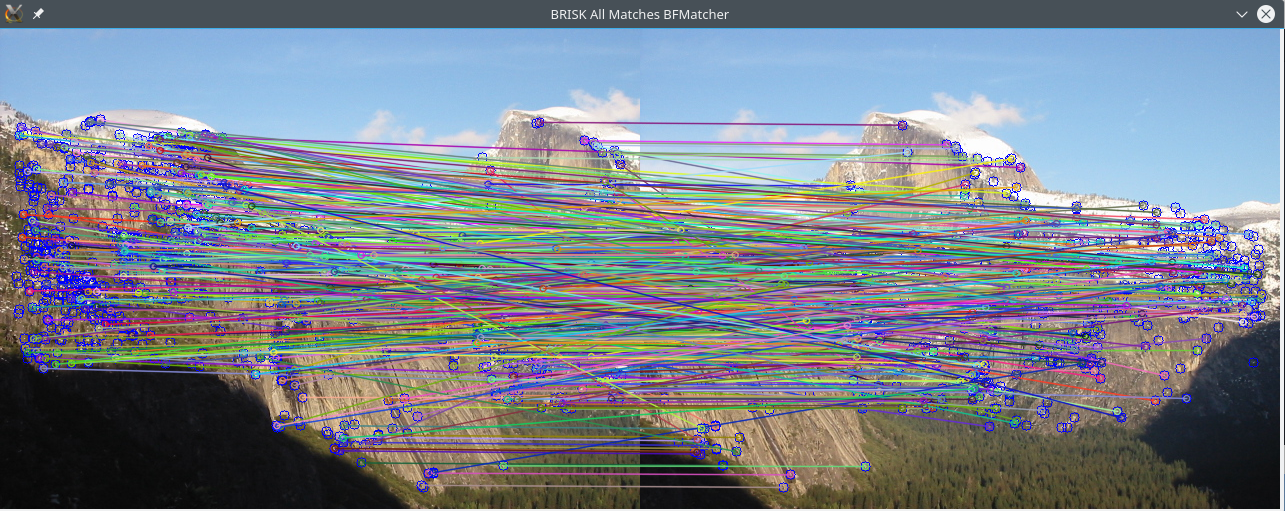
\includegraphics[width=0.7\textwidth]{BRISKBF.png}}
      \centerline{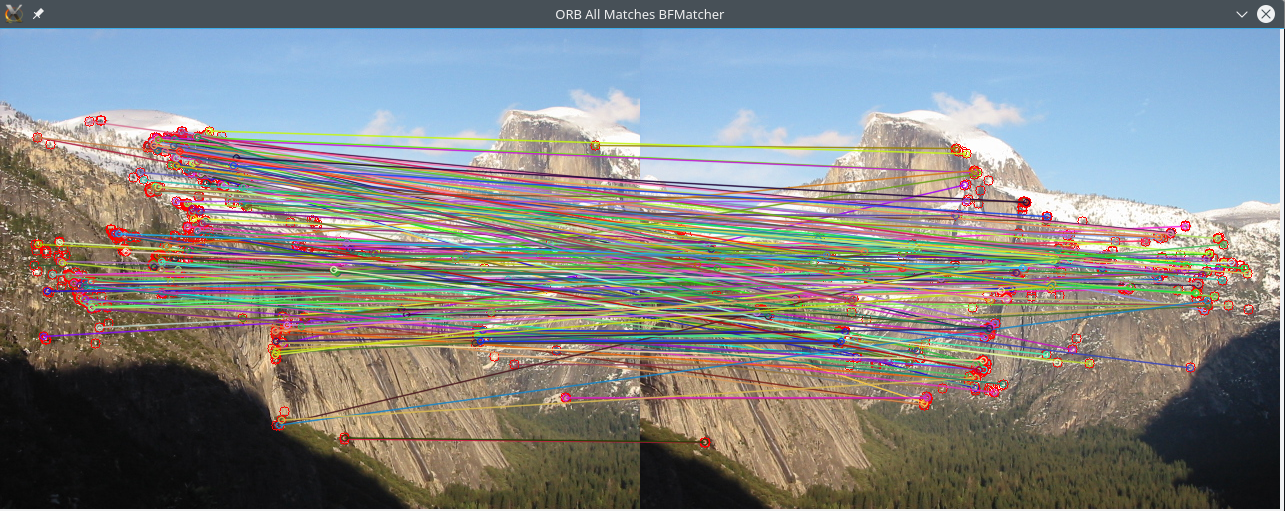
\includegraphics[width=0.7\textwidth]{ORBBF.png}}



      \centerline{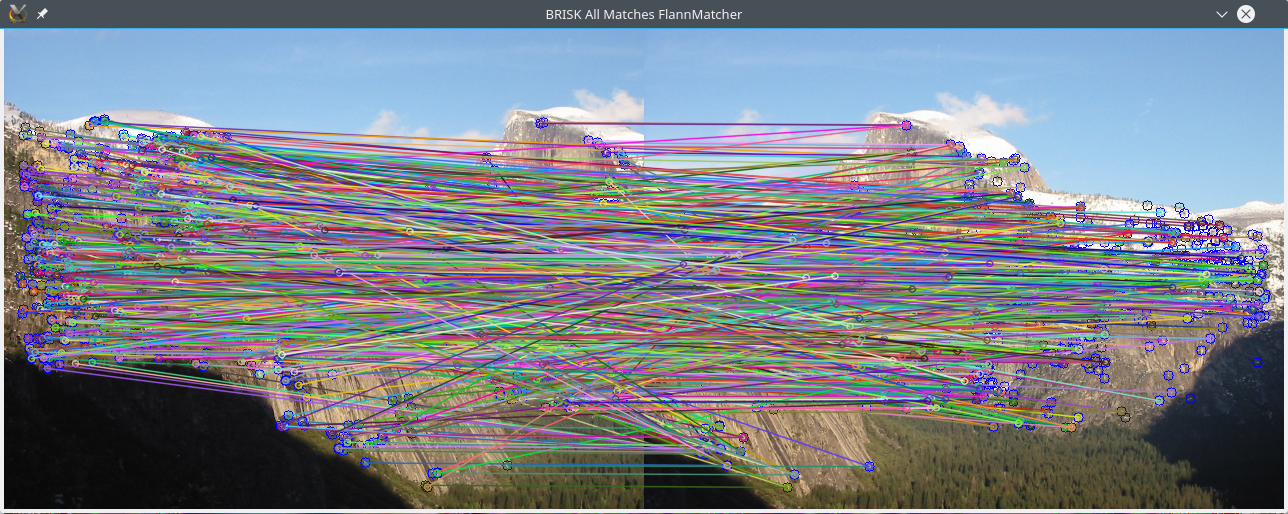
\includegraphics[width=0.7\textwidth]{BRISKFlann.png}}
      \centerline{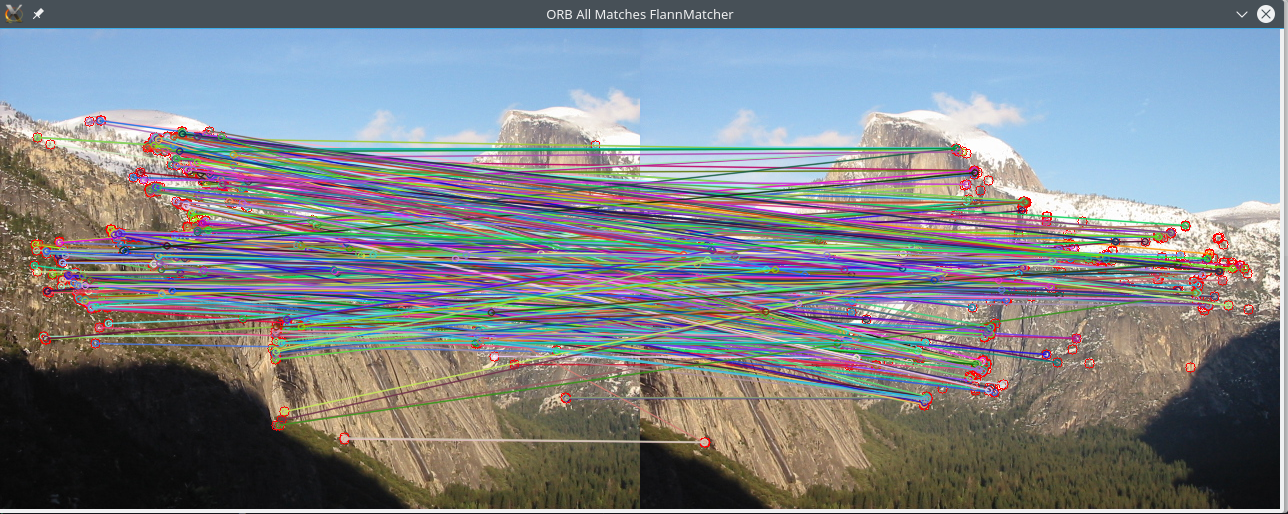
\includegraphics[width=0.7\textwidth]{ORBFlann.png}}

  \section {Creación de un panorama}

    Ahora por último sólo nos queda formar un panorama. En un principio se debe hacer
    para 2 imágenes y luego extrapolarlo a múltiples. Una vez estrapolado lo hemos añadido
    a la clase \textit{Image} como constructor de la clase, y sirve para un número cualquiera de imágenes.

    El método utiliza todo lo desarrollado arriba (eligiendo $BRISK$ y $BFMatcher$), supone que las imágenes están ordenadas,
    y una vez teniendo las correspondencias entre imágenes contiguas, hace lo siguiente:

    \begin{enumerate}
      \item Movemos la imagen central del panorama hacia dentro del canvas, dejando bastante hueco a los lados.
      \item Para cada imagen a la derecha de la central, se calcula su homografía adecuada y se coloca en el canvas.
      \item Restauramos la homografía inicial. Para cada imagen a la izquierda de la central, se calcula su homografía adecuada y se coloca en el canvas.
      \item Recortamos la imagen: Extraemos con el filtro de Canny los bordes y calculamos el rectángulo que los contiene.
    \end{enumerate}

    El filtro de Canny podría reducirse a un cálculo manual, usar la función \textit{threshold} para cada canal
    o usar \textit{inRange}. En cualquier caso el tiempo de programación no valdría la pena
    en relación a la ganancia que obtenemos, ya que las imágenes son pequeñas y utilizamos el filtro de Canny con
    los valores más permisivos. La función \textit{inRange} nos serviría si pudiéramos utilizar un intervalo abierto,
    ya que queremos cualquier valor distinto al (0,0,0).

    Los resultados obtenidos son los siguientes.

    \centerline{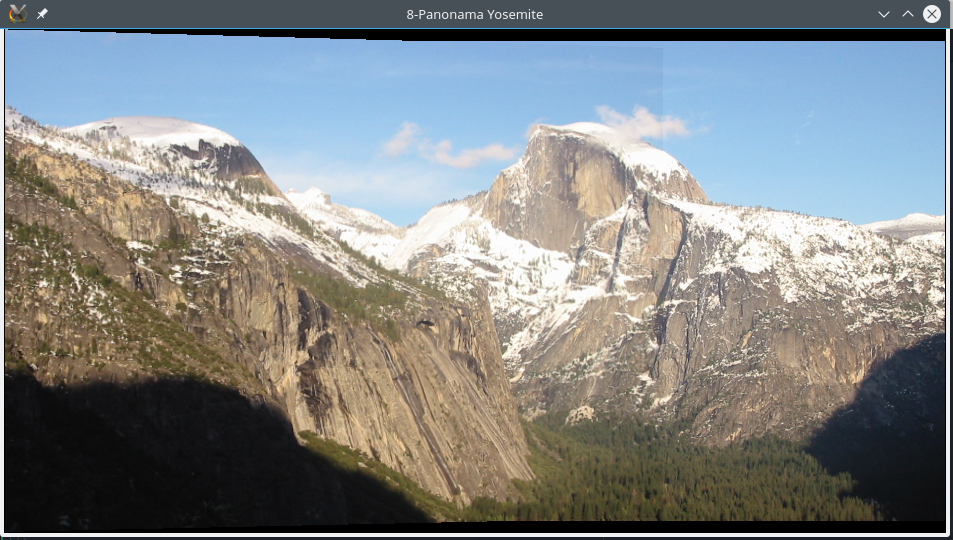
\includegraphics[width=0.7\textwidth]{YosemitePanorama.png}}
    \centerline{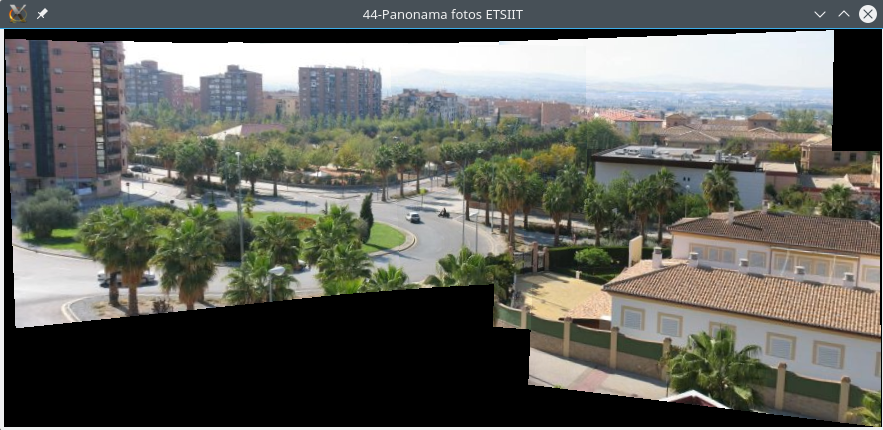
\includegraphics[width=0.7\textwidth]{ETSIITPanorama.png}}


\end{document}
